\documentclass[12pt]{article}
\usepackage[english]{babel}
\usepackage{natbib}
\usepackage{url}
\usepackage[utf8x]{inputenc}
\usepackage{amsmath}
\usepackage{graphicx}
\graphicspath{{img/}}
\usepackage{listings}
\usepackage{url}
\usepackage{parskip}
\usepackage{fancyhdr}
\usepackage{vmargin}
\usepackage{amssymb}
\usepackage{acronym}
\setmarginsrb{3 cm}{2.5 cm}{3 cm}{2.5 cm}{1 cm}{1.5 cm}{1 cm}{1.5 cm}

\title{Lab Report on \\Edge Detection and Image Compression }								% Title
\author{Rabi Raj Khadka}								% Author
\date{July 11, 2017}											% Date


\makeatletter
\let\thetitle\@title
\let\theauthor\@author
\let\thedate\@date
\makeatother

\pagestyle{fancy}
\fancyhf{}
\rhead{\theauthor}
\lhead{\thetitle}
\cfoot{\thepage}

\begin{document}
\begin{titlepage}
	\centering
   % \vspace*{0.5 cm}
    
\includegraphics[scale = 0.3]{kheclogo.jpg}\\[1.0 cm]	% University Logo
    \textsc{\LARGE Khwopa Engineering College}\\[1.5 cm]	% University Name
	\textsc{\Large Course Code :BEG 475 IP}\\[0.5 cm]				% Course Code
	\textsc{\large Image Processing and Pattern recogntiion}\\[0.5 cm]				% Course Name
	\rule{\linewidth}{0.2 mm} \\[0.4 cm]
	{ \huge \bfseries \thetitle}\\
	\rule{\linewidth}{0.2 mm} \\[1.0 cm]
	
	% \texttt{Lab Report \#1}
	
	\rule{\linewidth}{0 mm} \\[1.0 cm]

	\begin{minipage}{0.4\textwidth}
		\begin{flushleft} \large
			\emph{Author:}\\
			\theauthor
			\end{flushleft}
			\end{minipage}~
			\begin{minipage}{0.4\textwidth}
			\begin{flushright} \large
			\emph{Roll  Number:} \\
			700324									% Your Student Number
		\end{flushright}
	\end{minipage}\\[2cm]
	
	{\large \thedate}\\[2 cm]
 
	\vfill
	
\end{titlepage}
\tableofcontents
\pagebreak
\section{Theory}
\textbf{Edge Detection}\\
 Edge detection is a well-developed field on its own within image processing. Region boundaries and edges are closely related, since there is often a sharp adjustment in intensity at the region boundaries. Edge detection techniques have therefore been used as the base of another segmentation technique.\\

The edges identified by edge detection are often disconnected. To segment an object from an image however, one needs closed region boundaries. The desired edges are the boundaries between such objects or spatial-taxons.\\

Spatial-taxons are information granules, consisting of a crisp pixel region, stationed at abstraction levels within a hierarchical nested scene architecture. They are similar to the Gestalt psychological designation of figure-ground, but are extended to include foreground, object groups, objects and salient object parts. Edge detection methods can be applied to the spatial-taxon region, in the same manner they would be applied to a silhouette. This method is particularly useful when the disconnected edge is part of an illusory contour.\\

\texttt{Different Filters Used for Edge Detection are:}\\
$\rhd$\quad Gradient Filter\\
$\rhd$\quad Robert Filter\\
$\rhd$\quad Sobel Filter\\
$\rhd$\quad Prewitt Filter\\
$\rhd$\quad Canny Filter\\
$\rhd$\quad Laplace Filter\\

\pagebreak
\section{Code Description}
\emph{Program for Edge Detection and Compression }
\lstinputlisting[language=Matlab]{labsevenforreport.m}
\pagebreak
\section{Result and Discussion}
Input image is converted to gray scale image and gradient filter is applied to it and then robert filter on x axis and y axis alone are applied. Different Built-in fillters available on MATLAB is applied to grayscale image and shown as below.\\
Another image is taken for applying the Discrete Cosine Transformation and IDCT and image is compressed and saved as another image.\\
\emph{Outputs}\\
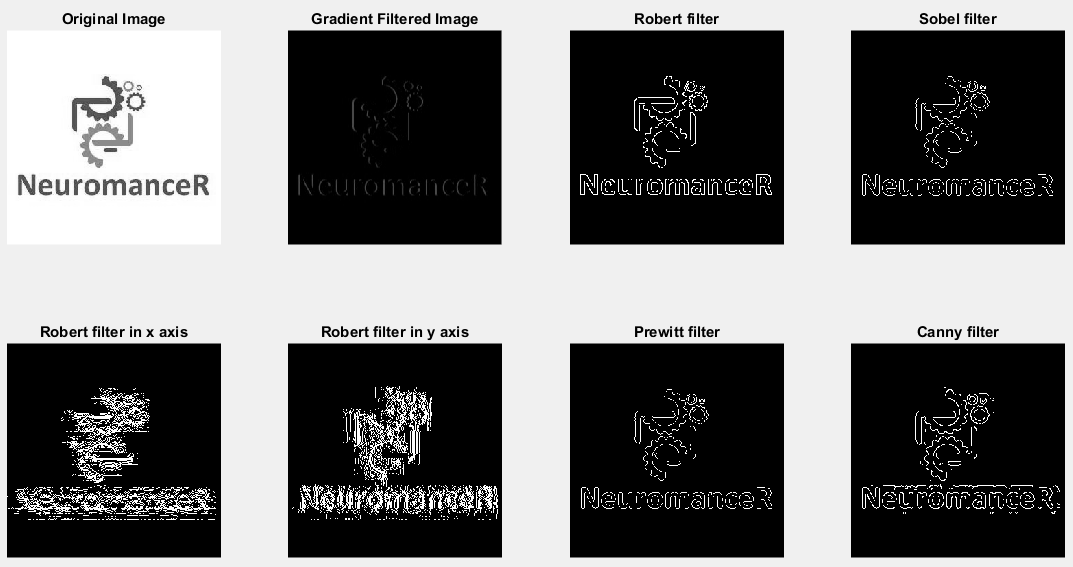
\includegraphics[scale = 0.4]{output_labseven_1.png}
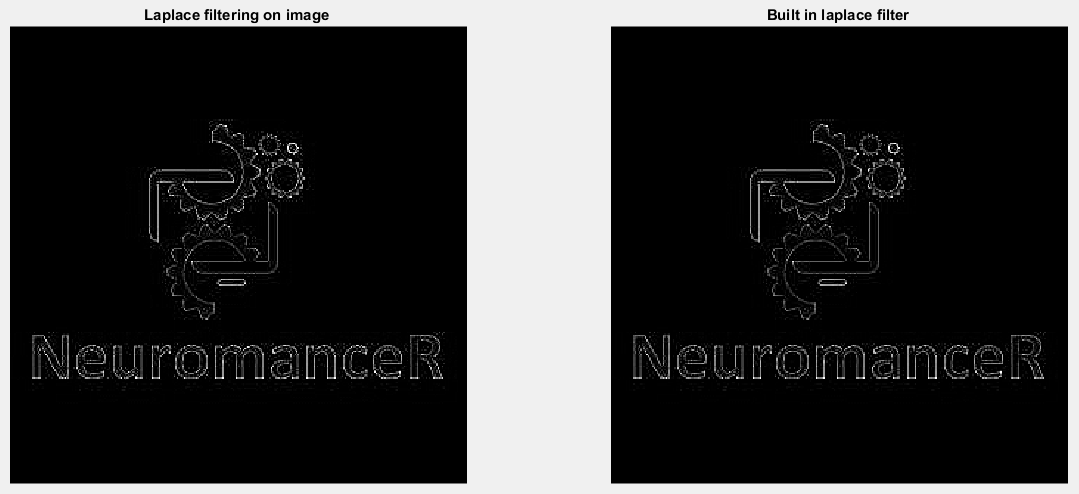
\includegraphics[scale = 0.2]{output_labseven_2.png}\\
\texttt{Figure 1:  Edge Detection Filters }\\

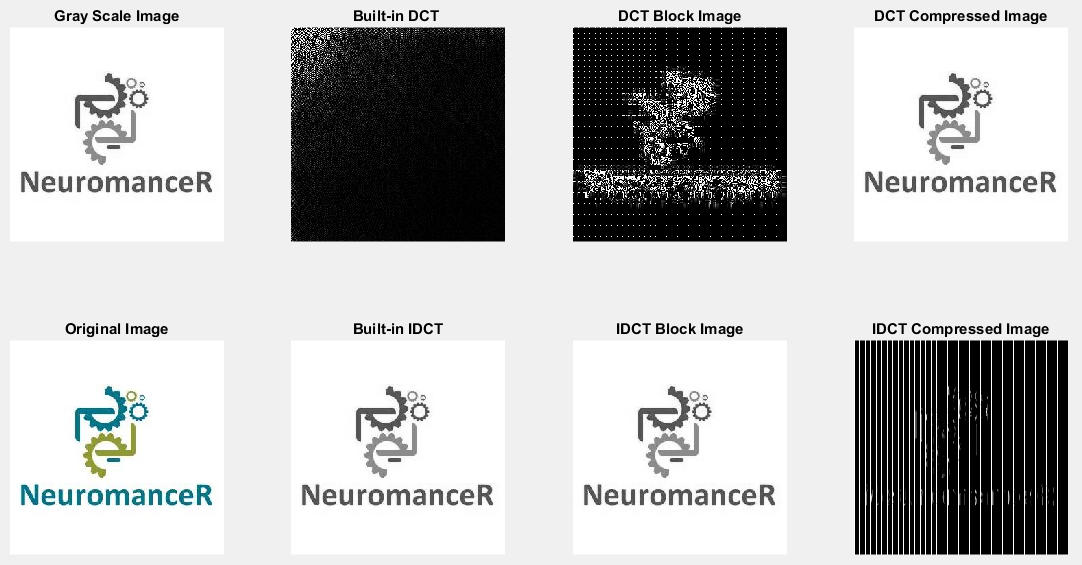
\includegraphics[scale = 0.4]{output_labseven_3.png}\\
\texttt{Figure 2: DCT and IDCT for Image Compression }\\

\pagebreak
\section{Conclusion}
Hence, \\
We are familiarized with edge detection of an image using different filters such as Sobel, Canny, Robert, Gradient,Laplace and Discrete Cosine Transformation and Inverse Discrete Cosine Transformation for image compression using the MATLAB application.
\end{document}